\chapter{Приложения}
\label{ch:appendix}

\section{Приложение А. Теоретический вывод формул}

Рассмотрим подзадачу о диффузии в соединительной трубке. Предположим сперва, что концентрации примеси (гелия) на её торцах поддерживаются постоянными и равными $n_1$ и $n_2$ соответственно. Тогда через некоторое время (оценку этого времени см. ниже формулу (9)) в трубке установится стационарный поток частиц, одинаковый в каждом сечении трубки (в противном случае, если бы поток зависел от $x$, частицы бы накапливались в трубке, и процесс перестал бы быть стационарным).

Применяя закон Фика в трубке, получим:
\begin{equation}
j = -D \pdv{n}{x} = \text{const}
\end{equation}

Следовательно, распределение концентрации в трубке $n(x)$ -- линейная функция:
\begin{equation}
n(x) = \frac{\Delta n}{L} x
\end{equation}
и плотность потока частиц всюду постоянна и равна
\begin{equation}
j = -D \frac{\Delta n}{L}
\end{equation}
где $\Delta n = n_2 - n_1$ -- разность концентраций гелия на концах трубки.

Теперь вернёмся к процессу выравнивания концентраций в сосудах. Частицы перетекают из сосуда 2 в сосуд 1 по трубке, и концентрации $n_1(t)$ и $n_2(t)$ меняются во времени. Предположим, что этот процесс происходит достаточно медленно, так что в трубке в любой момент времени успевает установиться практически стационарное течение, описываемое формулами (3), (4). Такое приближение называют \emph{квазистационарным}.

Кроме того, будем считать, что в пределах каждого сосуда частицы распределены равномерно, так что концентрации примеси вблизи трубки и в остальных частях сосуда отличаются мало. Тогда полное число частиц примеси в сосудах равно соответственно $N_1 = n_1V$ и $N_2 = n_2V$. Произведение плотности потока (4) на площадь сечения трубки $S$ даёт количество частиц, пересекающих в единицу времени любое поперечное сечение трубки. Поэтому
\begin{equation}
\dv{N_1}{t} = jS, \quad \dv{N_2}{t} = -jS
\end{equation}

Выразим отсюда скорость изменения $\Delta n$. Вычитая из второго равенства первое и деля результат на объём сосуда $V$, с учетом (4) получим
\begin{equation}
\dv{(\Delta n)}{t} = -\frac{\Delta n}{\tau}
\end{equation}
где введено обозначение
\begin{equation}
\tau = \frac{1}{D} \frac{VL}{2S}
\end{equation}

Интегрируя (6), получаем, что разность концентраций будет убывать по экспоненциальному закону
\begin{equation}
\Delta n = \Delta n_0 e^{-t/\tau}
\end{equation}
где $\Delta n_0$ -- разность концентраций примеси в сосудах в начальный момент времени. Видно, что величина $\tau$ есть характерное время выравнивания концентраций между сосудами. Оно определяется геометрическими размерами установки и коэффициентом диффузии.

\section{Приложение Б. Ход работы}
    
\subsection{Подготовка установки к работе}
а) включили питание датчиков и измерительного моста;

б) убедились, что кран подачи гелия К7 плотно закрыт, и в установке нет
запертых объёмов

в) подсоединили установку к форвакуумному насосу и откачали её до давления
~0.1 торр. Это достигается непрерывной работой насоса в течение
3–5 минут (при этом показания манометра M, измеряющего разность
давление между установкой и атмосферой, достигли максимума);

г) после окончания откачки выключили насос.

\subsection{Балансировка измерительного моста при рабочем давлении}

Для начала выберем $P_{\Sigma} = 40~\text{торр}$

а) напустили в установку воздух до давления $P_{\Sigma}$;

б) изолировали рабочие объёмы, закрыв краны К1, К2 (К3 открыт);

в) cбалансировали измерительный мост так, чтобы показания вольтметра флуктуировали в среднем около нулевого значения. Использовали последовательно ручки регулировки «грубо», затем «точно». После балансировки и до окончания измерений при данном $P_{\Sigma}$ положения ручек регулировки не меняли. Удалось добиться флуктуаций значений напряжения в пределах $0.01~\text{мВ}$.

\subsection{Приготовление рабочих смесей}

В сосуде $V_2$ должен оказаться чистый воздух, в $V_1$ смесь воздуха с гелием. Давления в сосудах должны быть одинаковы и равны рабочему $P_{\Sigma}$. Для этого выполнили следующие действия:

а) Откачали всю установку до $\approx 0.1~\text{торр}$.

б) Изолировали объём $V_2$, закрыв краны К2 и К3. После этого остановили откачку.

в) Напустили в установку гелий до давления $P_{He} = 0.1P_{\Sigma}$. После этого изолировали объём $V_1$ (краном К1).

г) Перекрыли подачу гелия (кран К7) и откачали гелий из всех патрубков. Затем остановили откачку.

д) Присоединили объём $V_2$ к установке (кран К2) и заполнили всю установку, исключая объём $V_1$, воздухом (без гелия) до давления, избыточного по сравнению с планируемым рабочим давлением ($1.675P_{\Sigma}$).

е) Уравняли давления в сосудах $V_1$ и $V_2$, создав поток из сосуда с воздухом в сосуд с гелием. Для этого открыли краны K1 и K2 при закрытых K3 и K4. Поскольку газ при адиабатическом расширении остывает, необходимо держать краны К1 и К2 открытыми в течение некоторого времени (30–60 с), чтобы дать давлениям выравняться при одинаковых температурах. Это время не должно быть слишком велико, чтобы диффузия гелия по патрубкам в обратном направлении не привела к искажению приготовленного состояния.

ж) Записали точное значение установившегося рабочего давления $P_{\Sigma} = 40~\text{торр}$. Изолировали объёмы $V_1$ и $V_2$, перекрыв краны К1 и К2. Система должна быть готова к измерениям.

\subsection{Измерение изменения теплопроводности}

Процесс диффузии начался после открывания крана К3 . Прежде приготовили компьютерную программу по дополнительному описанию. Открыли К3 и измерили, как меняются показания вольтметра с течением времени. Измерение продолжали до тех пор, пока напряжение не упало на 50\%.

\subsection{Измерения при различных значениях рабочего давления}

Повторили измерения пп. 3–5 при различных значениях рабочего давления в диапазоне 40–200 торр (всего 5 значений). Графики, полученные при измерениях приведены в приложении.

\section{Приложение В. Параметры установки}

Номер установки - 1. Схема на рисунке \ref{ustanovka}.

\begin{figure}[ht]
    \center{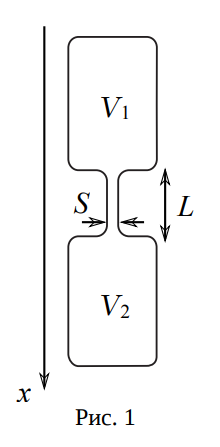
\includegraphics[scale=0.75]{img/ustanovka.png}}
   
    \label{ustanovka}
\end{figure}
 \begin{center}
        Рис. 1. Схема установки. Для исследования взаимной диффузии газов и измерения коэффициента взаимной диффузии D использовались два сосуда объёмами $V_1$ и $V_2$ ($V_1 \approx V_2 \equiv V $), заполненные гелием и воздухом при одинаковом давлении, но с различной концентрацией компонентов. Сосуды соединены трубкой длины $L$ и сечения $S$. Чтобы считать концентрации газов $n_1$ и $n_2$ внутри каждого сосуда постоянными по всему объёму и принять, что процесс выравниваний концентраций происходил благодаря диффузии в трубке, использовалась соединительная трубка с малым объёмом по сравнению с объёмом сосудов. Геометрические размеры установки и коэффициент взаимной диффузии гелия и воздуха определяют характерное время выравнивания концентраций между сосудами.  %(полностью описание) для чего, что на рисунке
    \end{center}
    
Геометрические характеристики установки:\\
    $V_1 = V_2 = V = (775 \pm 10)~\text{см}^3$,\\
    $\frac{L}{S} = (5.3 \pm 0.1)~\text{см}^{-1}$.\\
Атмосферное давление и цена деления вакууметра:
    $P_{\text{атм}} = 760~\text{торр}$,\\
    $\text{Ц. Д. вакуумметра} = 7.43~\text{торр}$.

\section{Приложение Г. Результаты измерений}

\begin{figure}[ht]
    \centering
        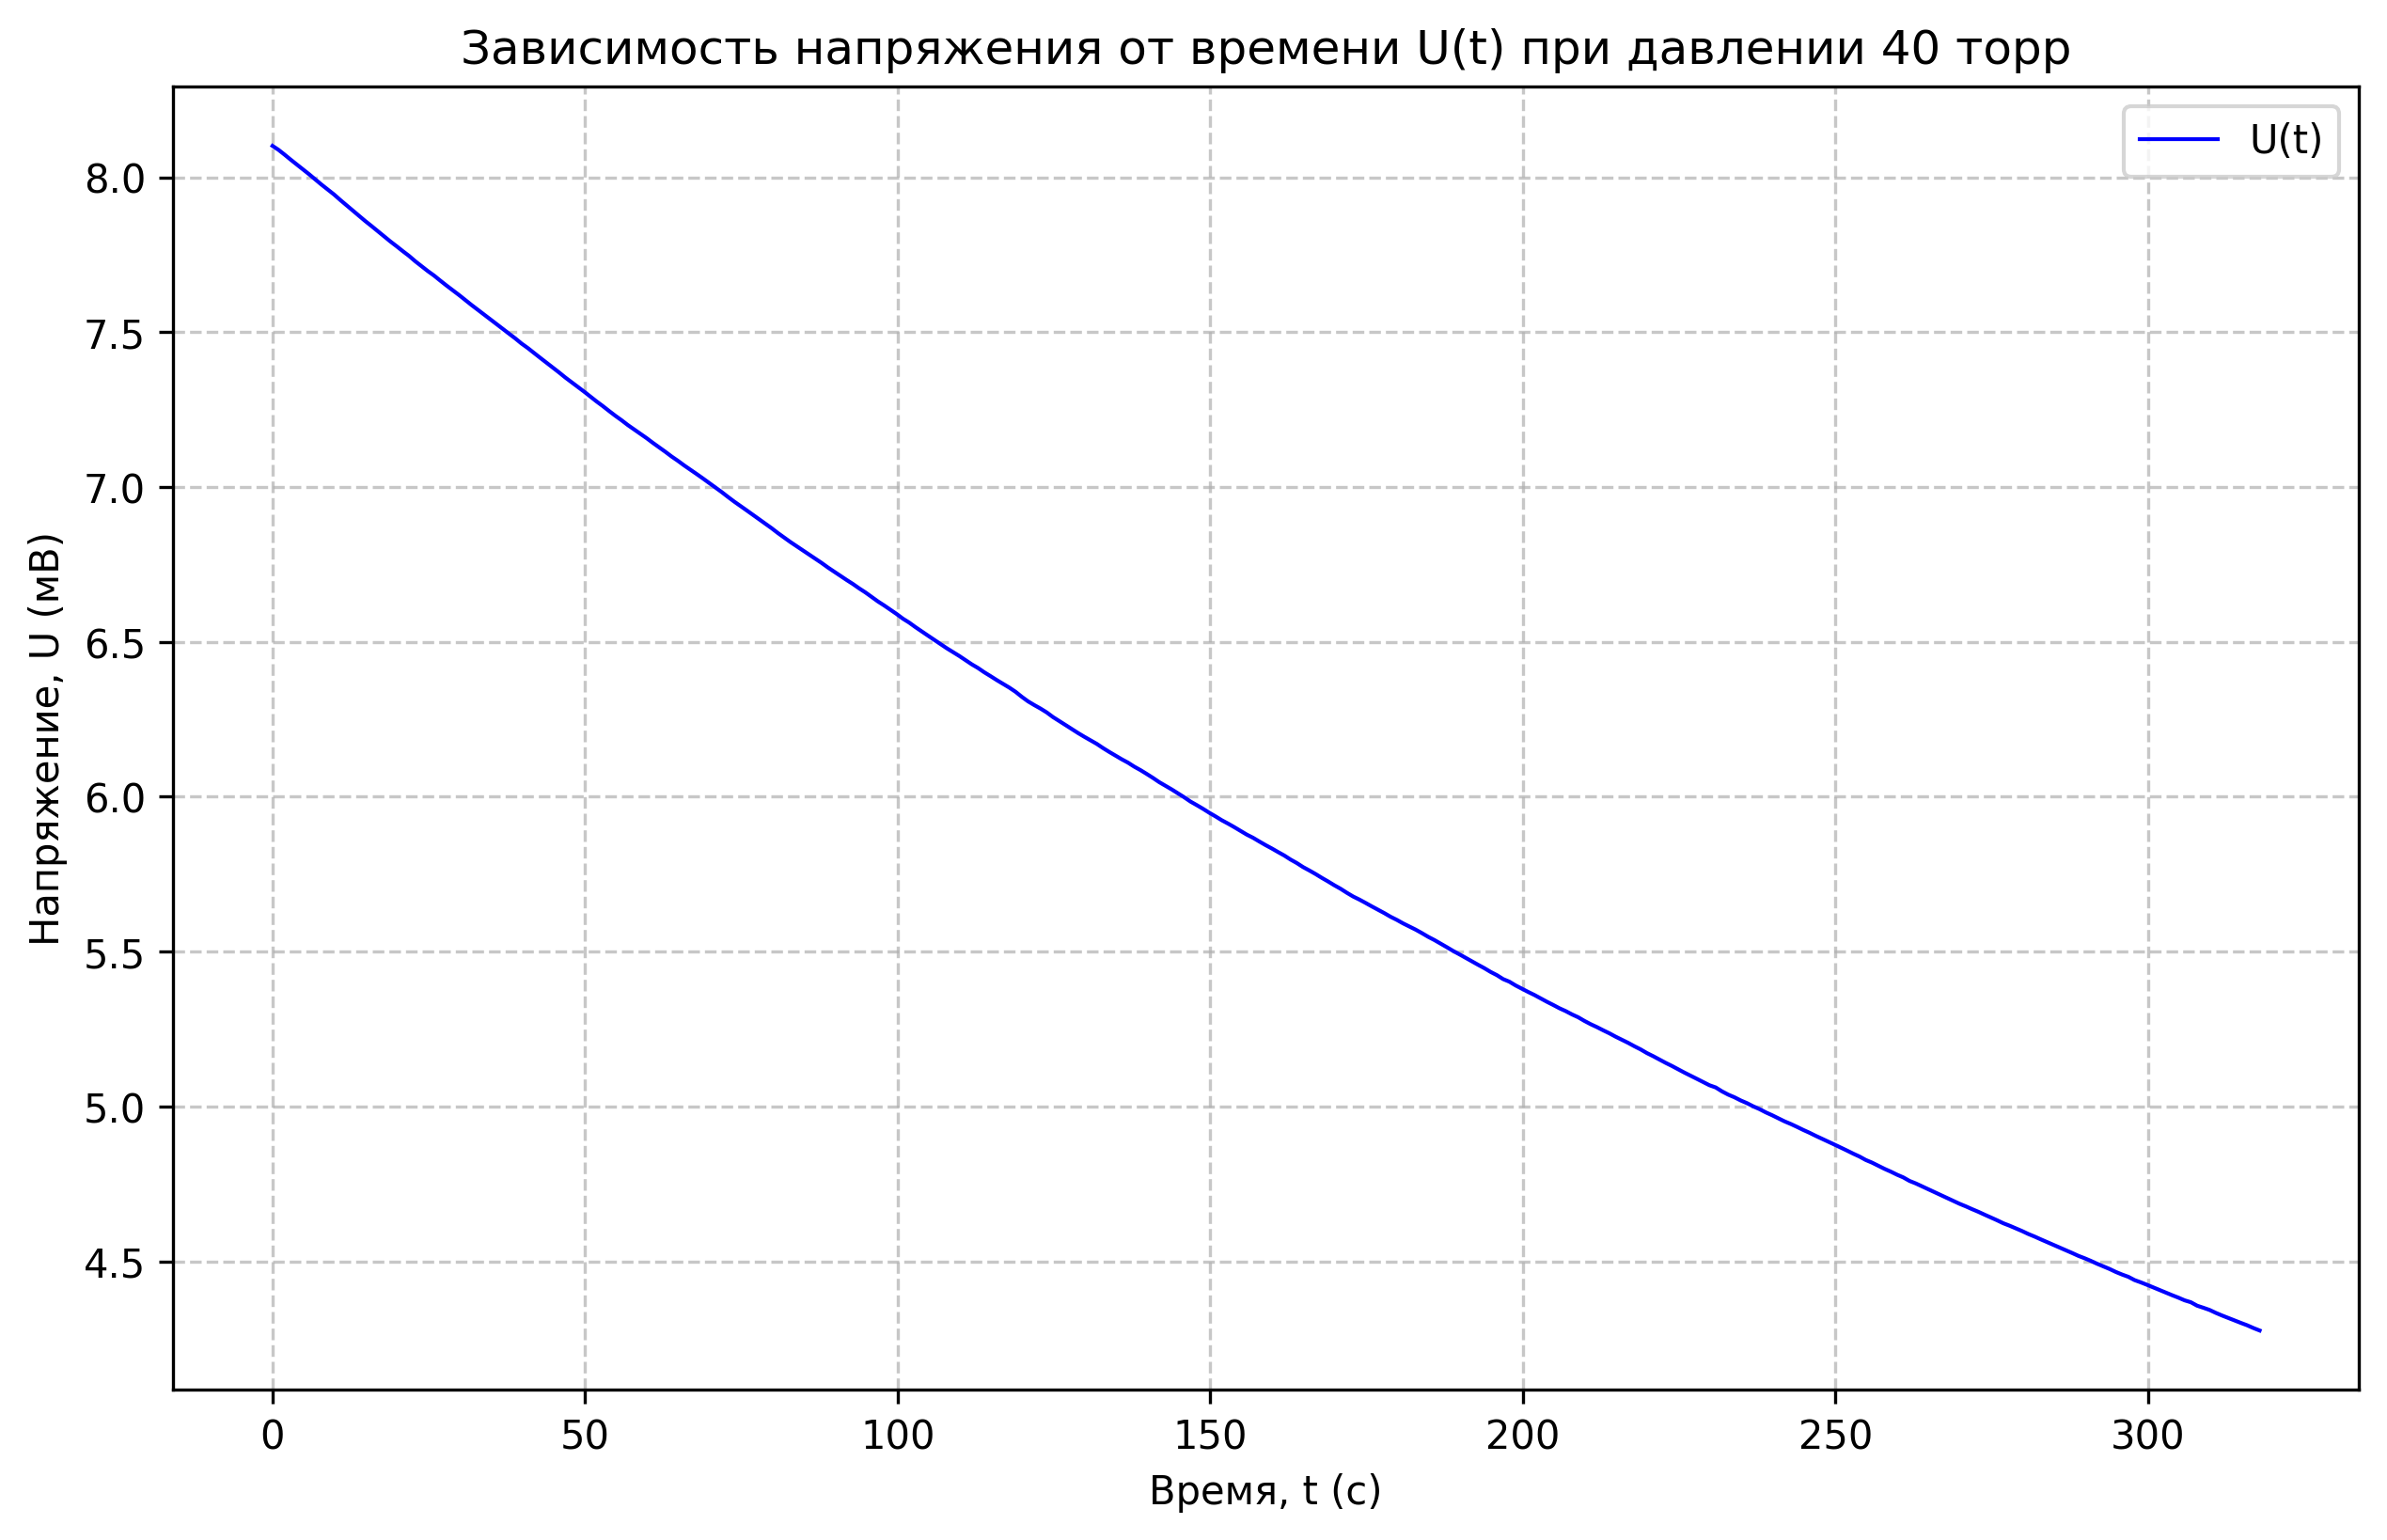
\includegraphics[width = \textwidth]{img/40.png}
Рис. 4. Зависимость напряжения от времени при давлении 40 торр.     
\end{figure}

\begin{figure}[ht]
    \centering
        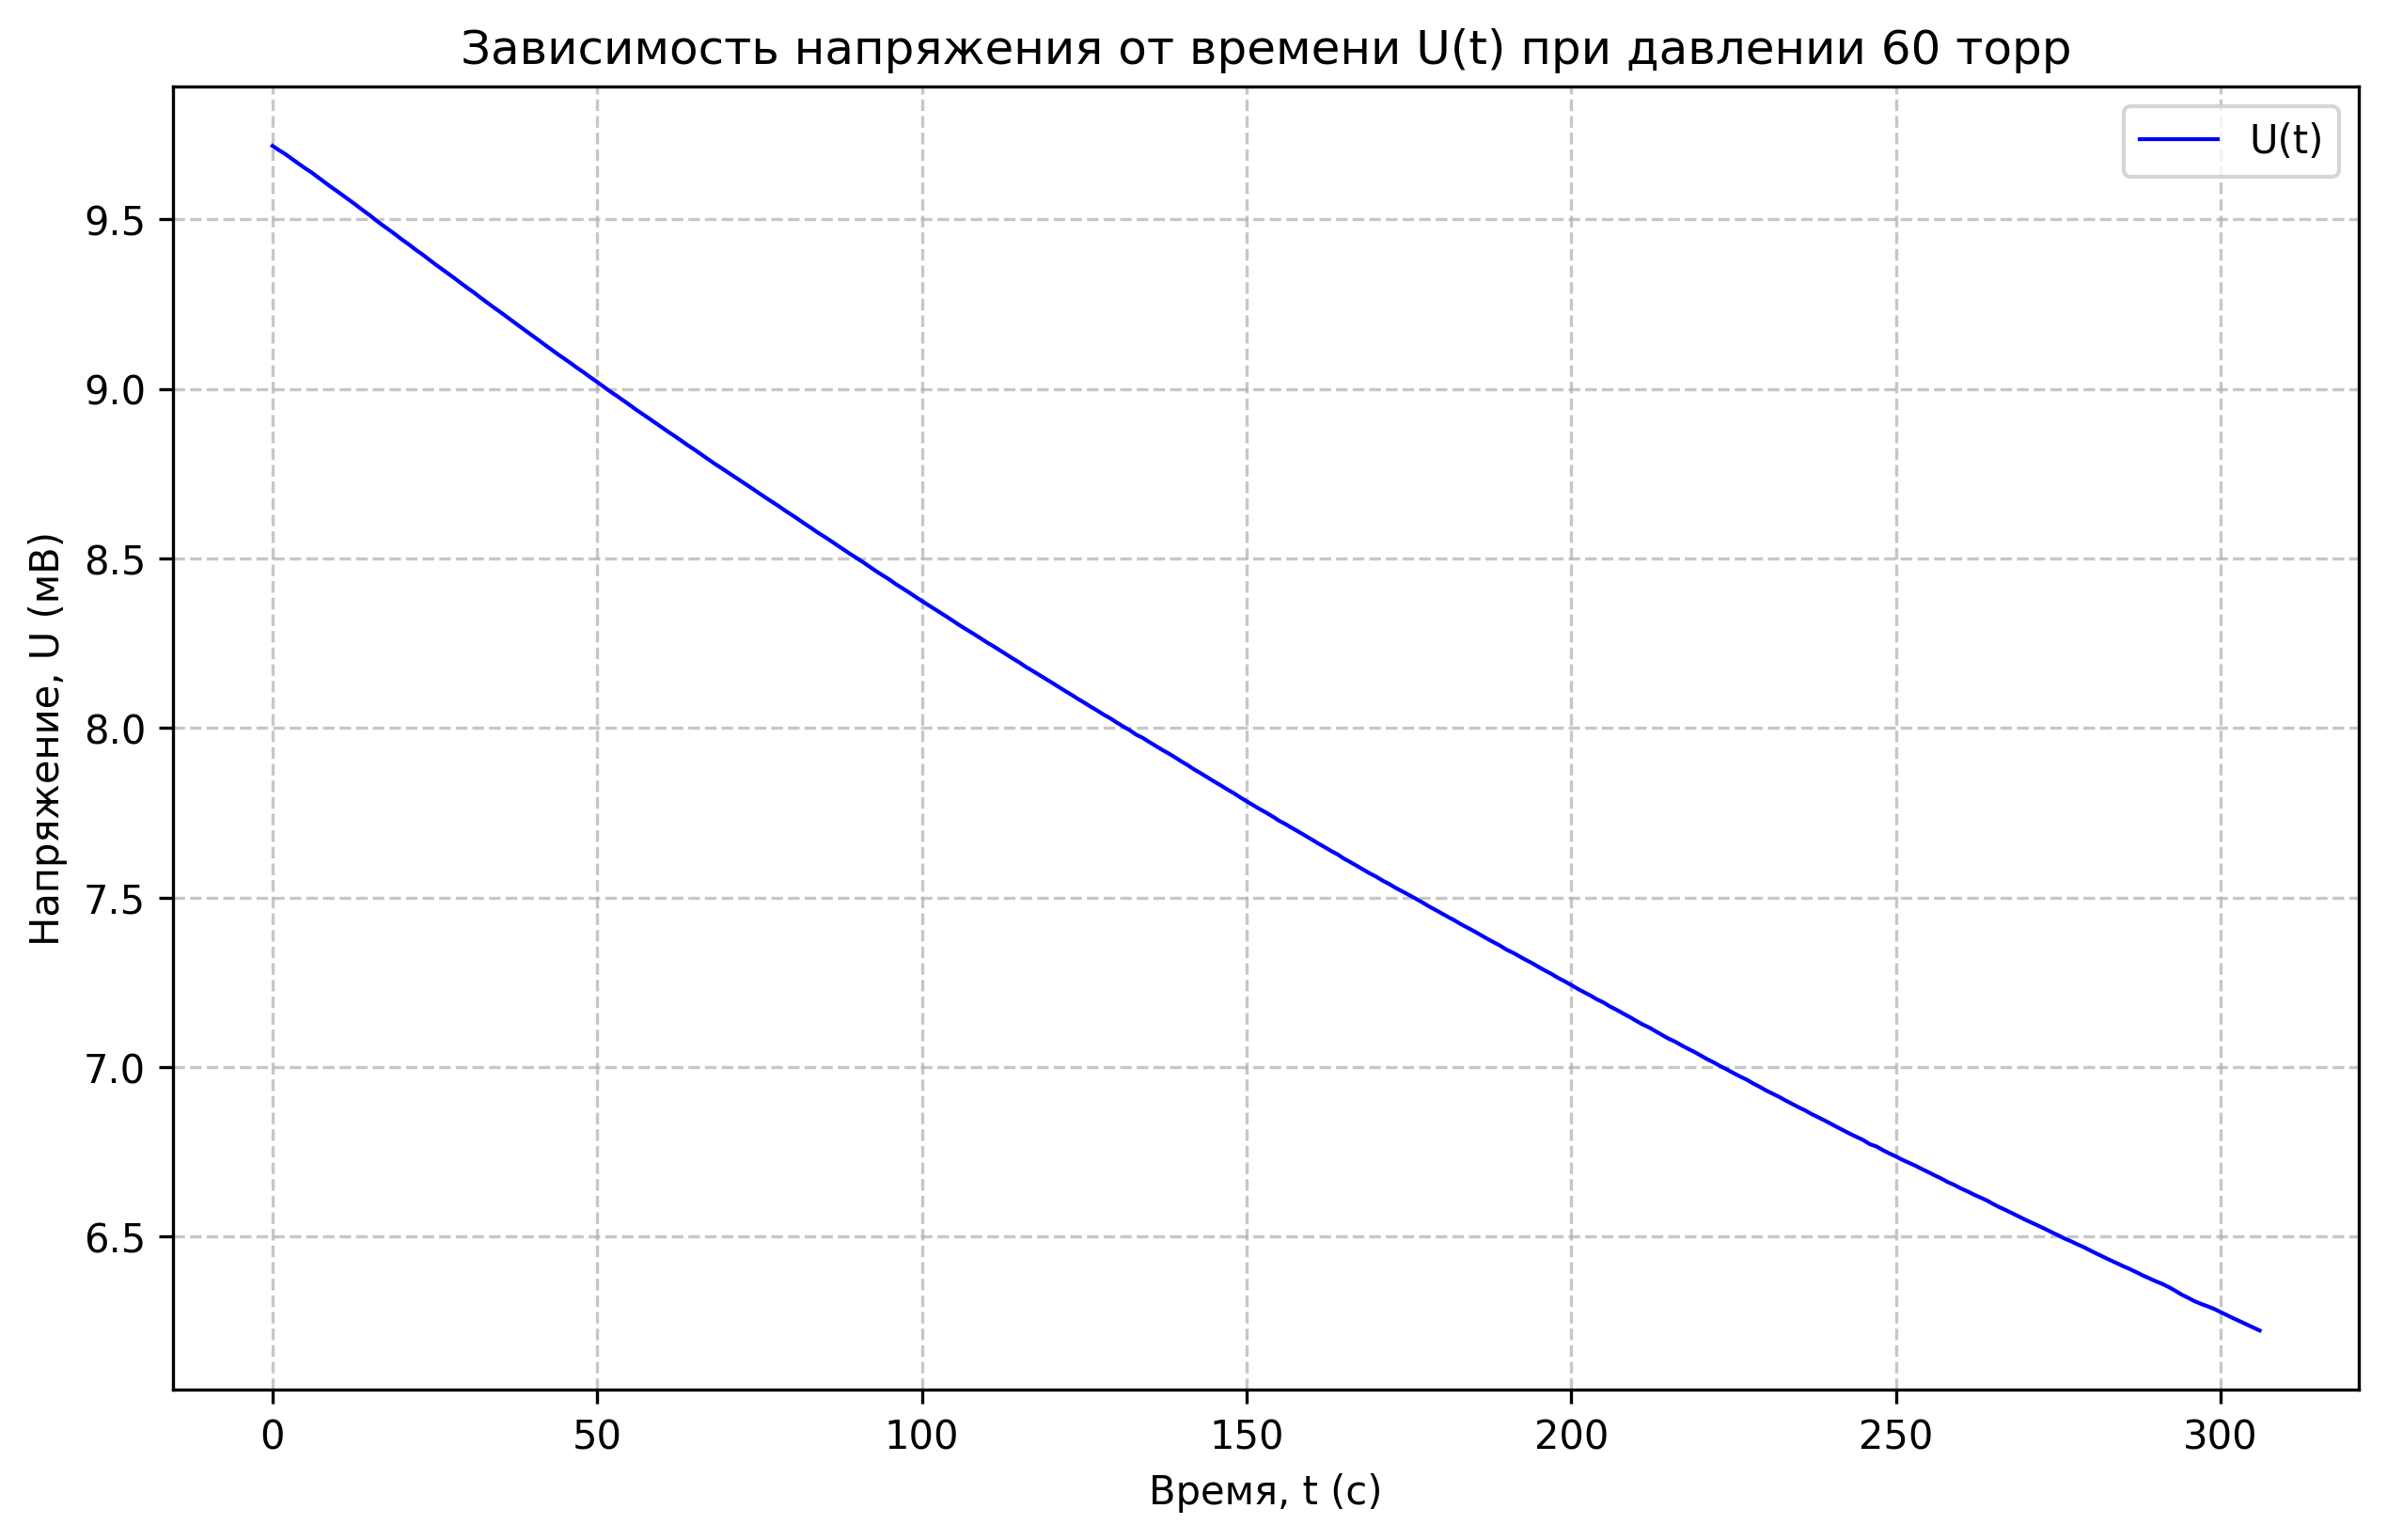
\includegraphics[width = \textwidth]{img/60.png}
Рис. 5. Зависимость напряжения от времени при давлении 60 торр.   
\end{figure}


\begin{figure}[ht]
    \centering
        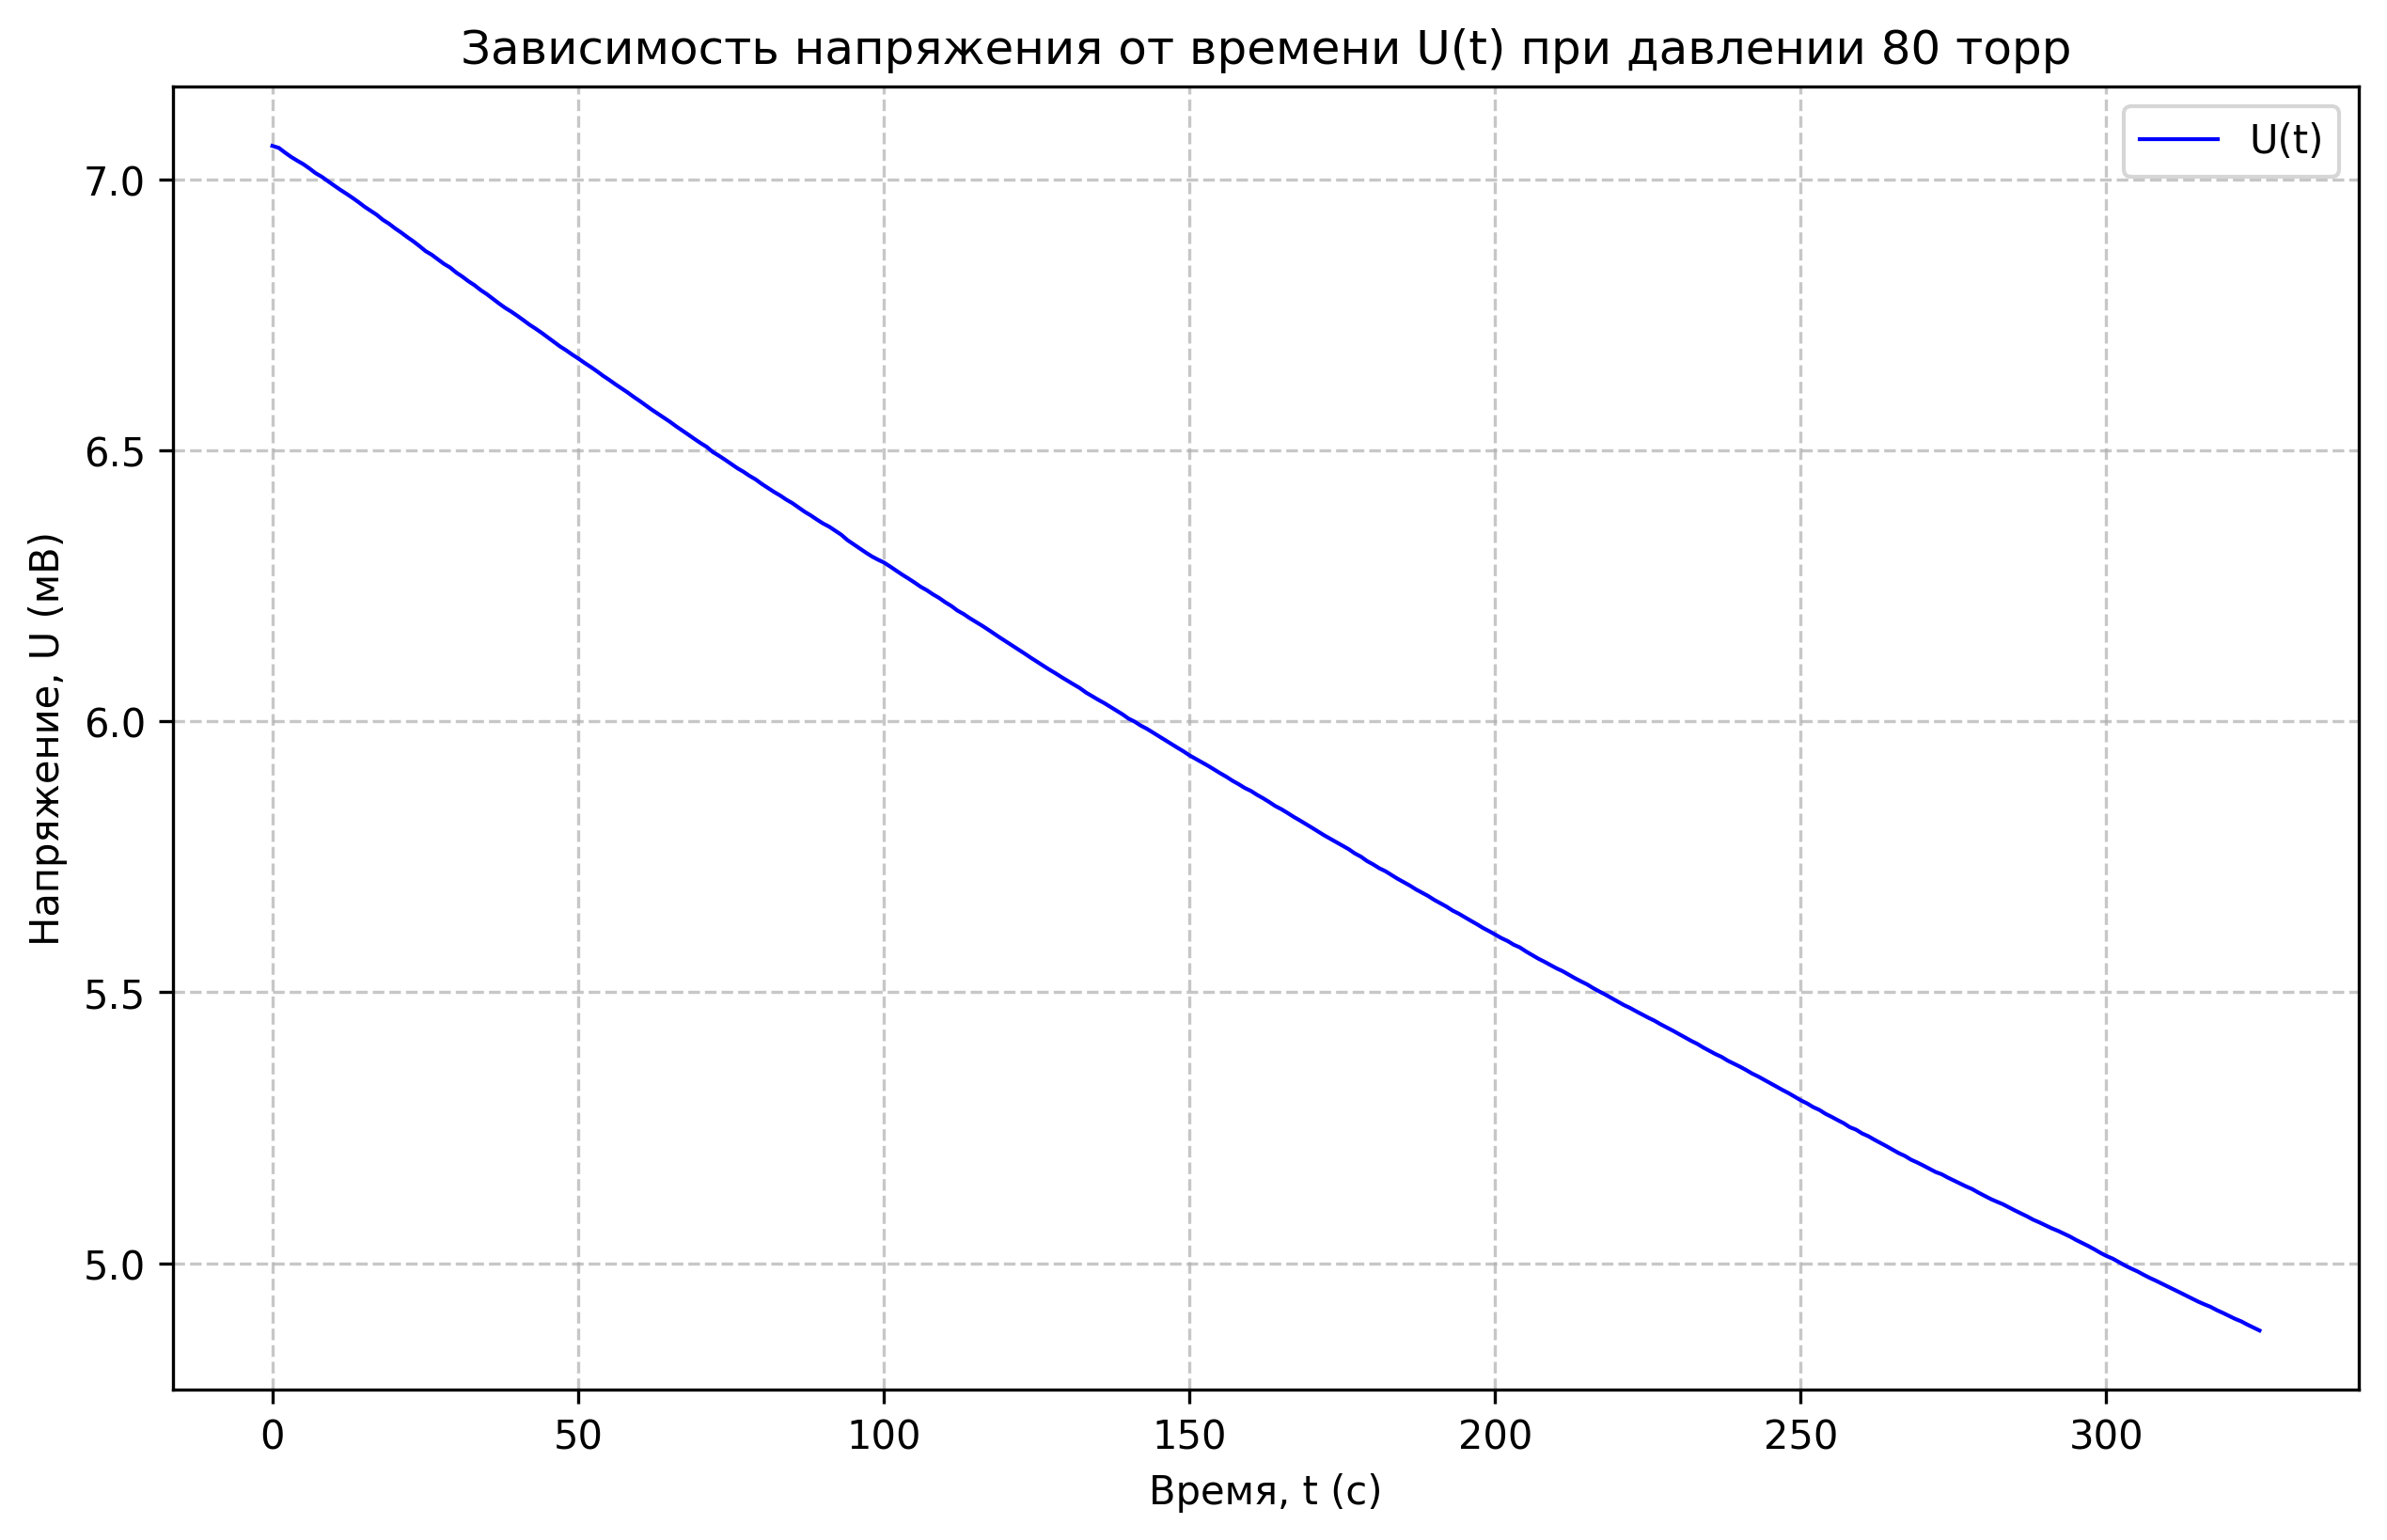
\includegraphics[width = \textwidth]{img/80.png}
Рис. 6. Зависимость напряжения от времени при давлении 80 торр.    
\end{figure}

\begin{figure}[ht]
    \centering
        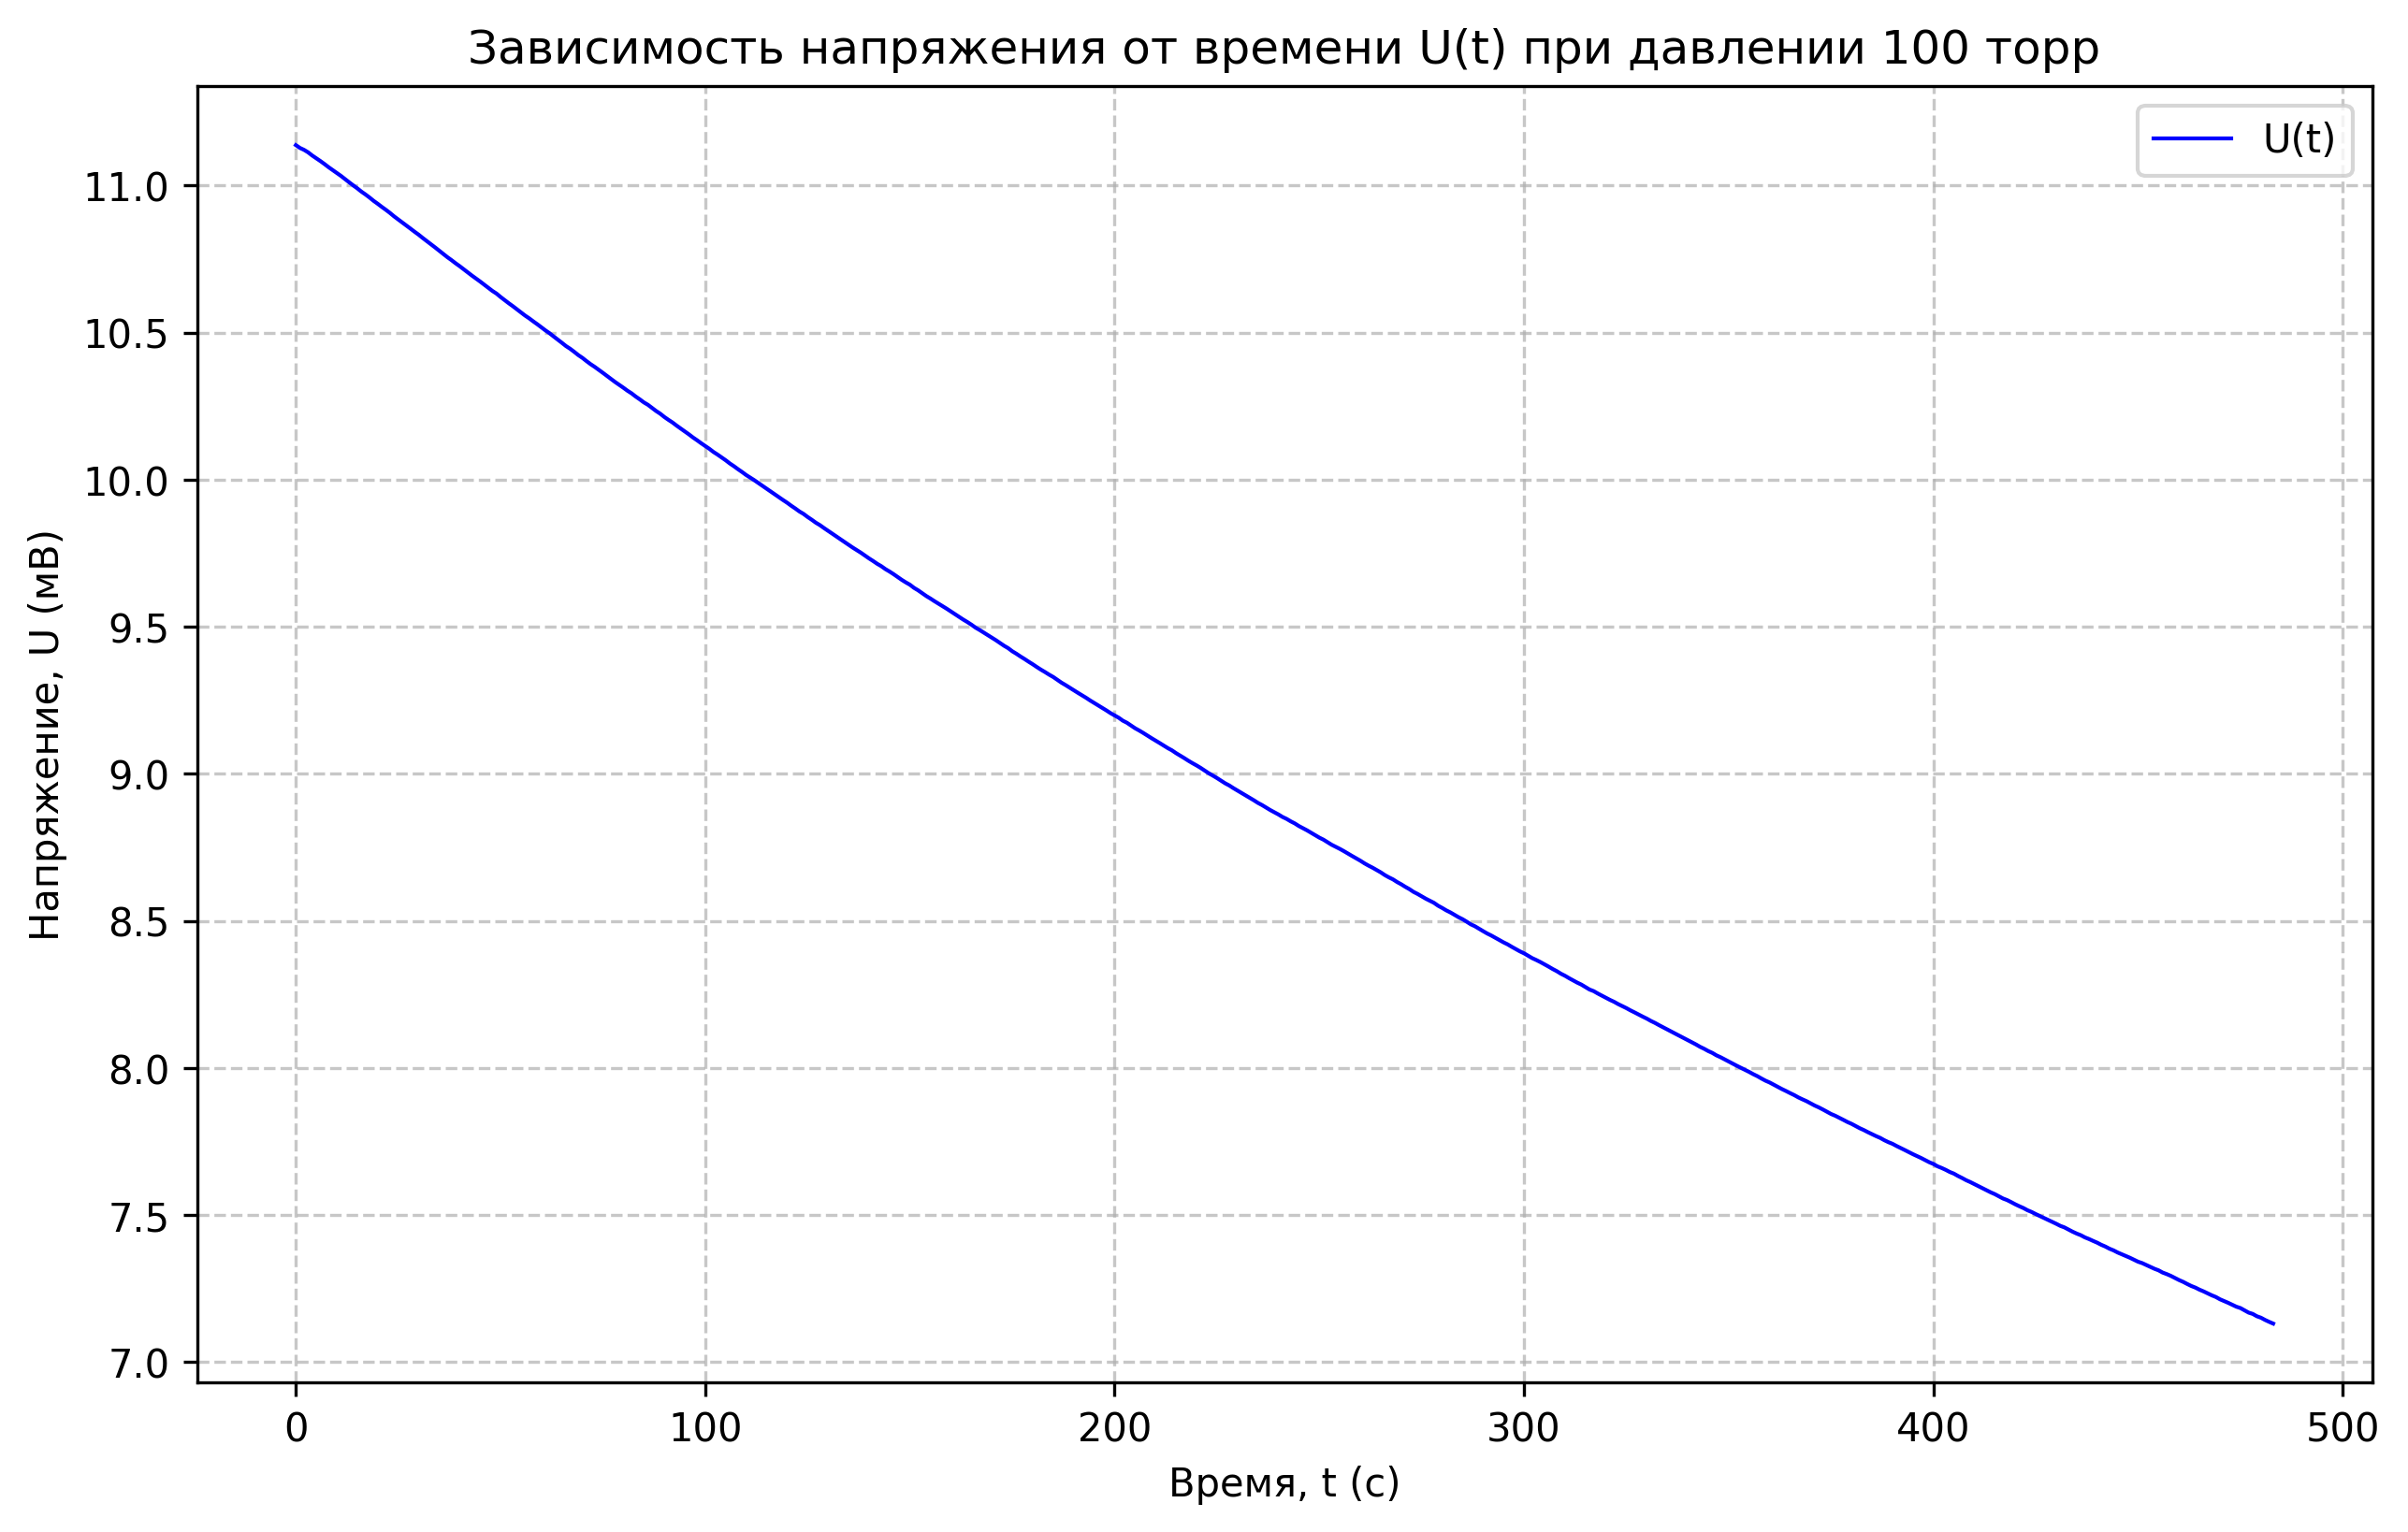
\includegraphics[width = \textwidth]{img/100.png}
Рис. 7. Зависимость напряжения от времени при давлении 100 торр.  
\end{figure}


\begin{figure}[ht]
    \centering
        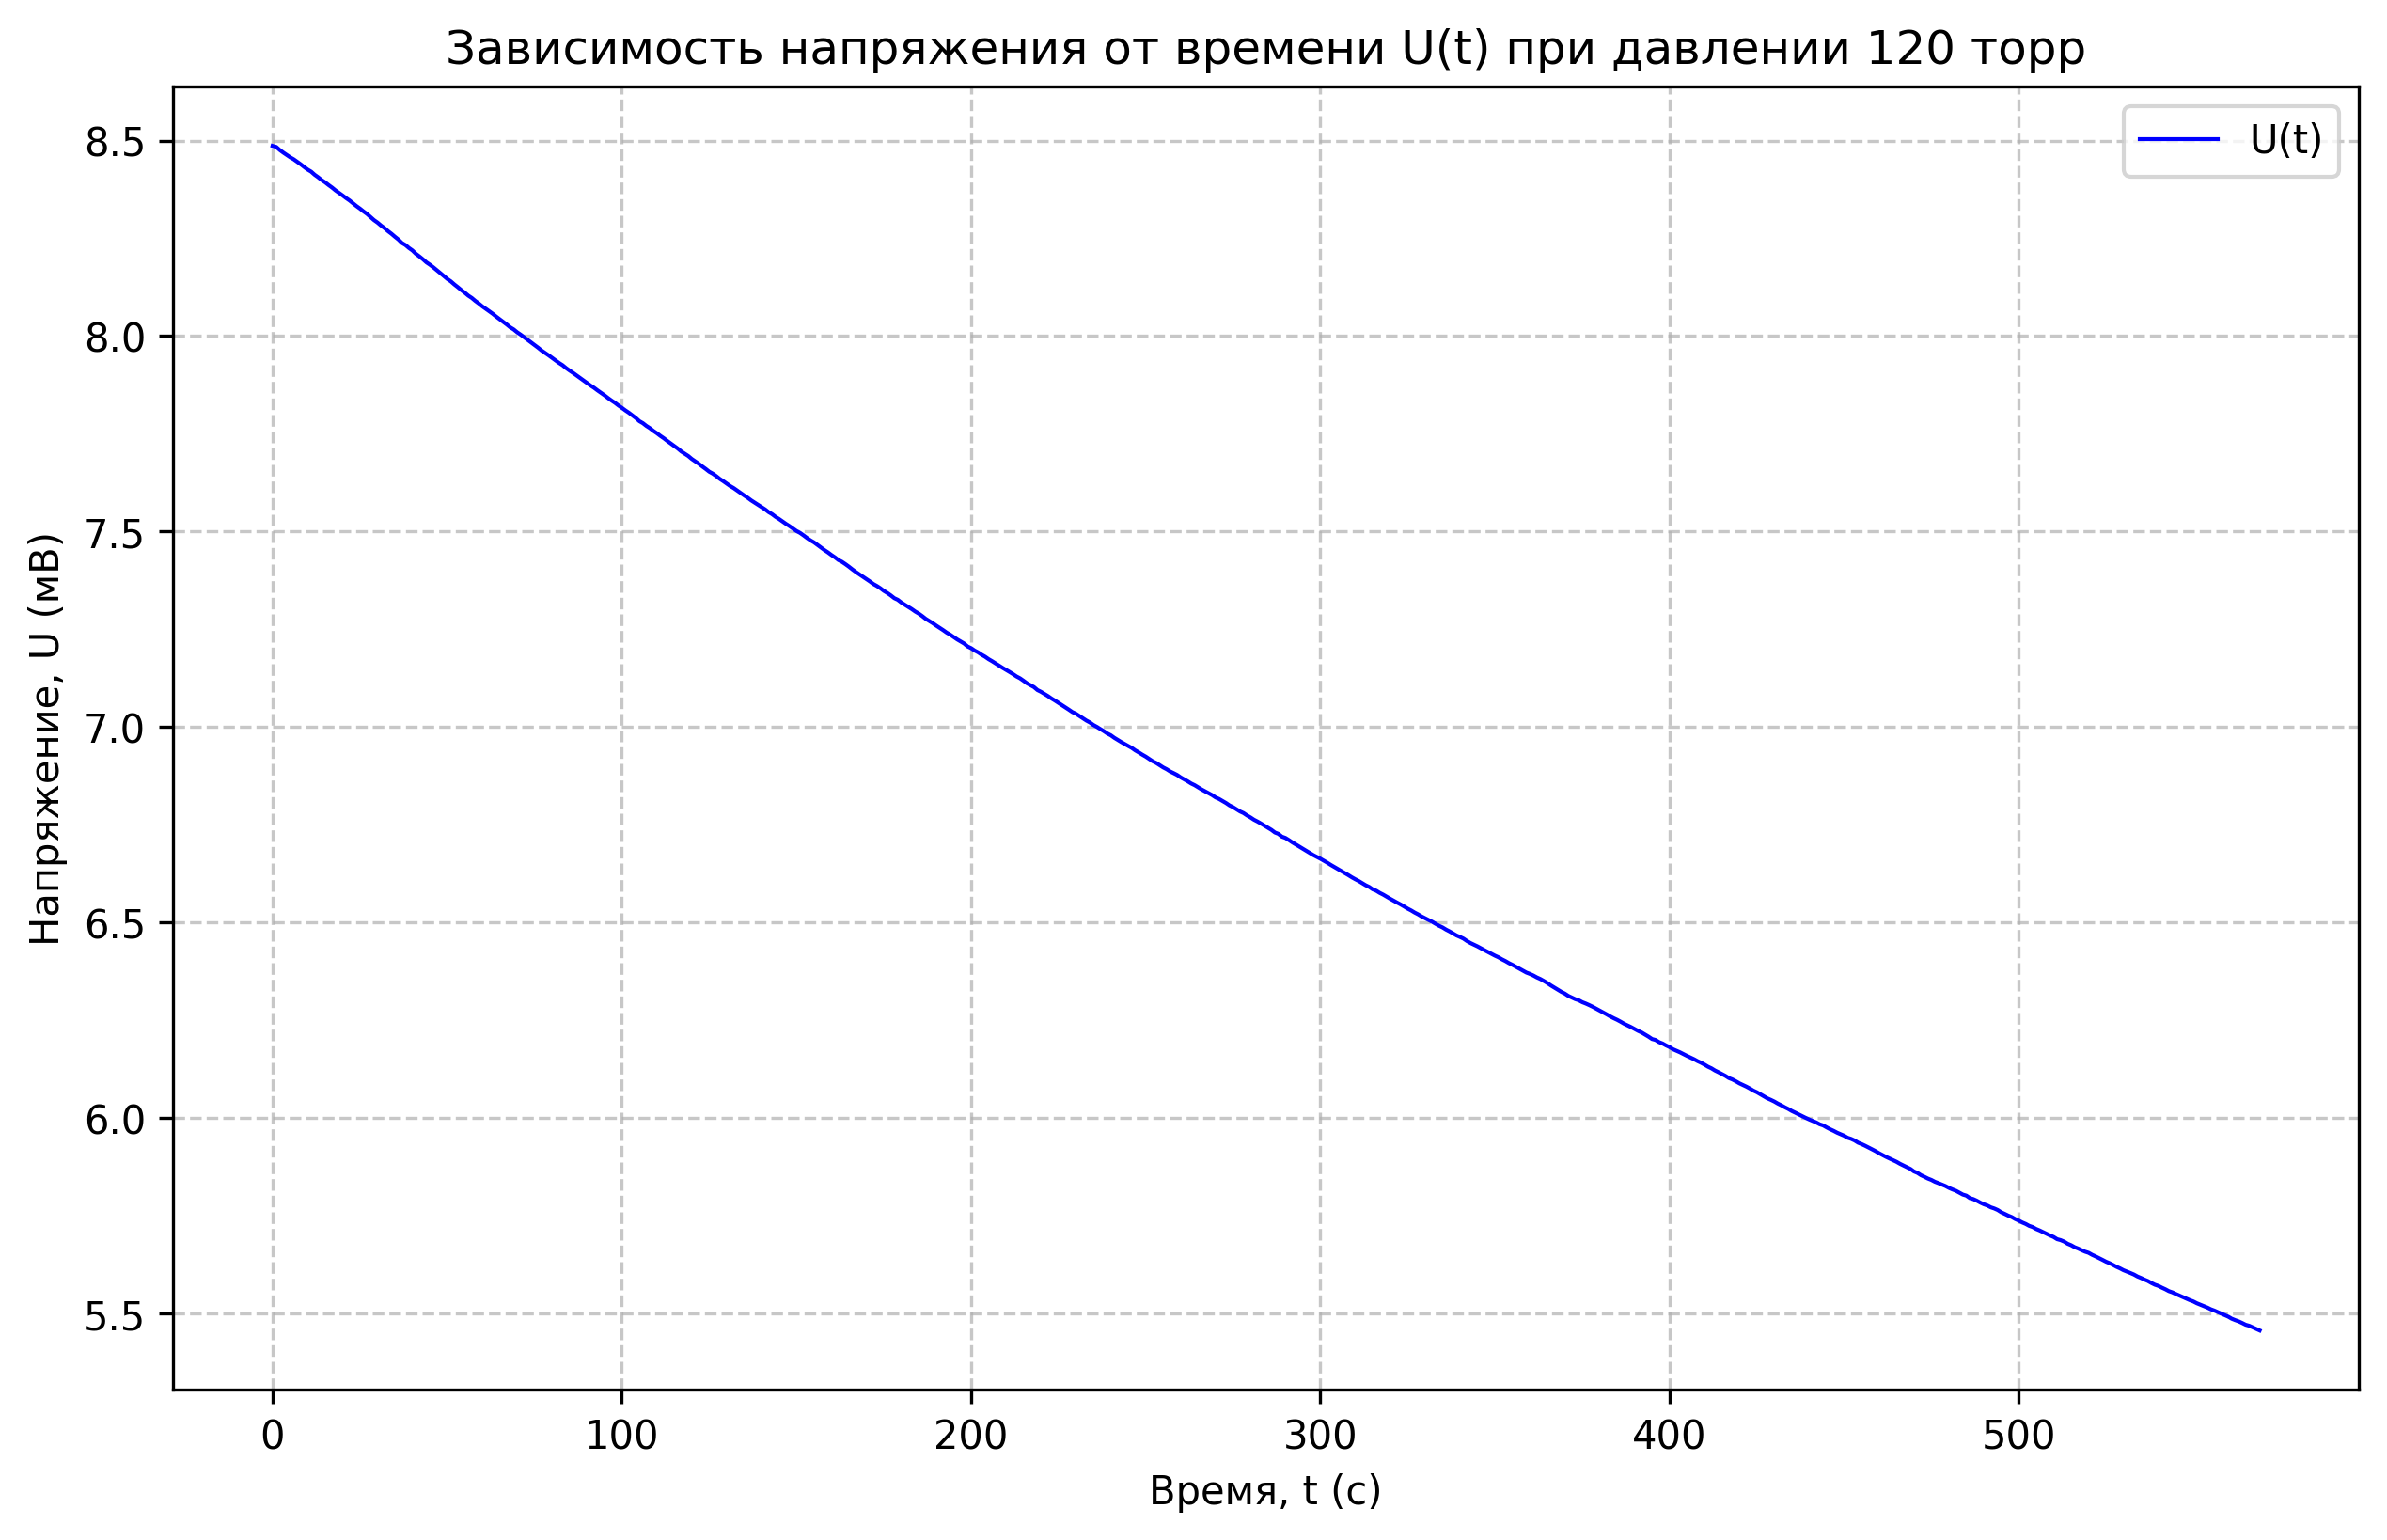
\includegraphics[width = \textwidth]{img/120.png}
Рис. 8. Зависимость напряжения от времени при давлении 120 торр.    
\end{figure}


\begin{figure}[ht]
    \centering
        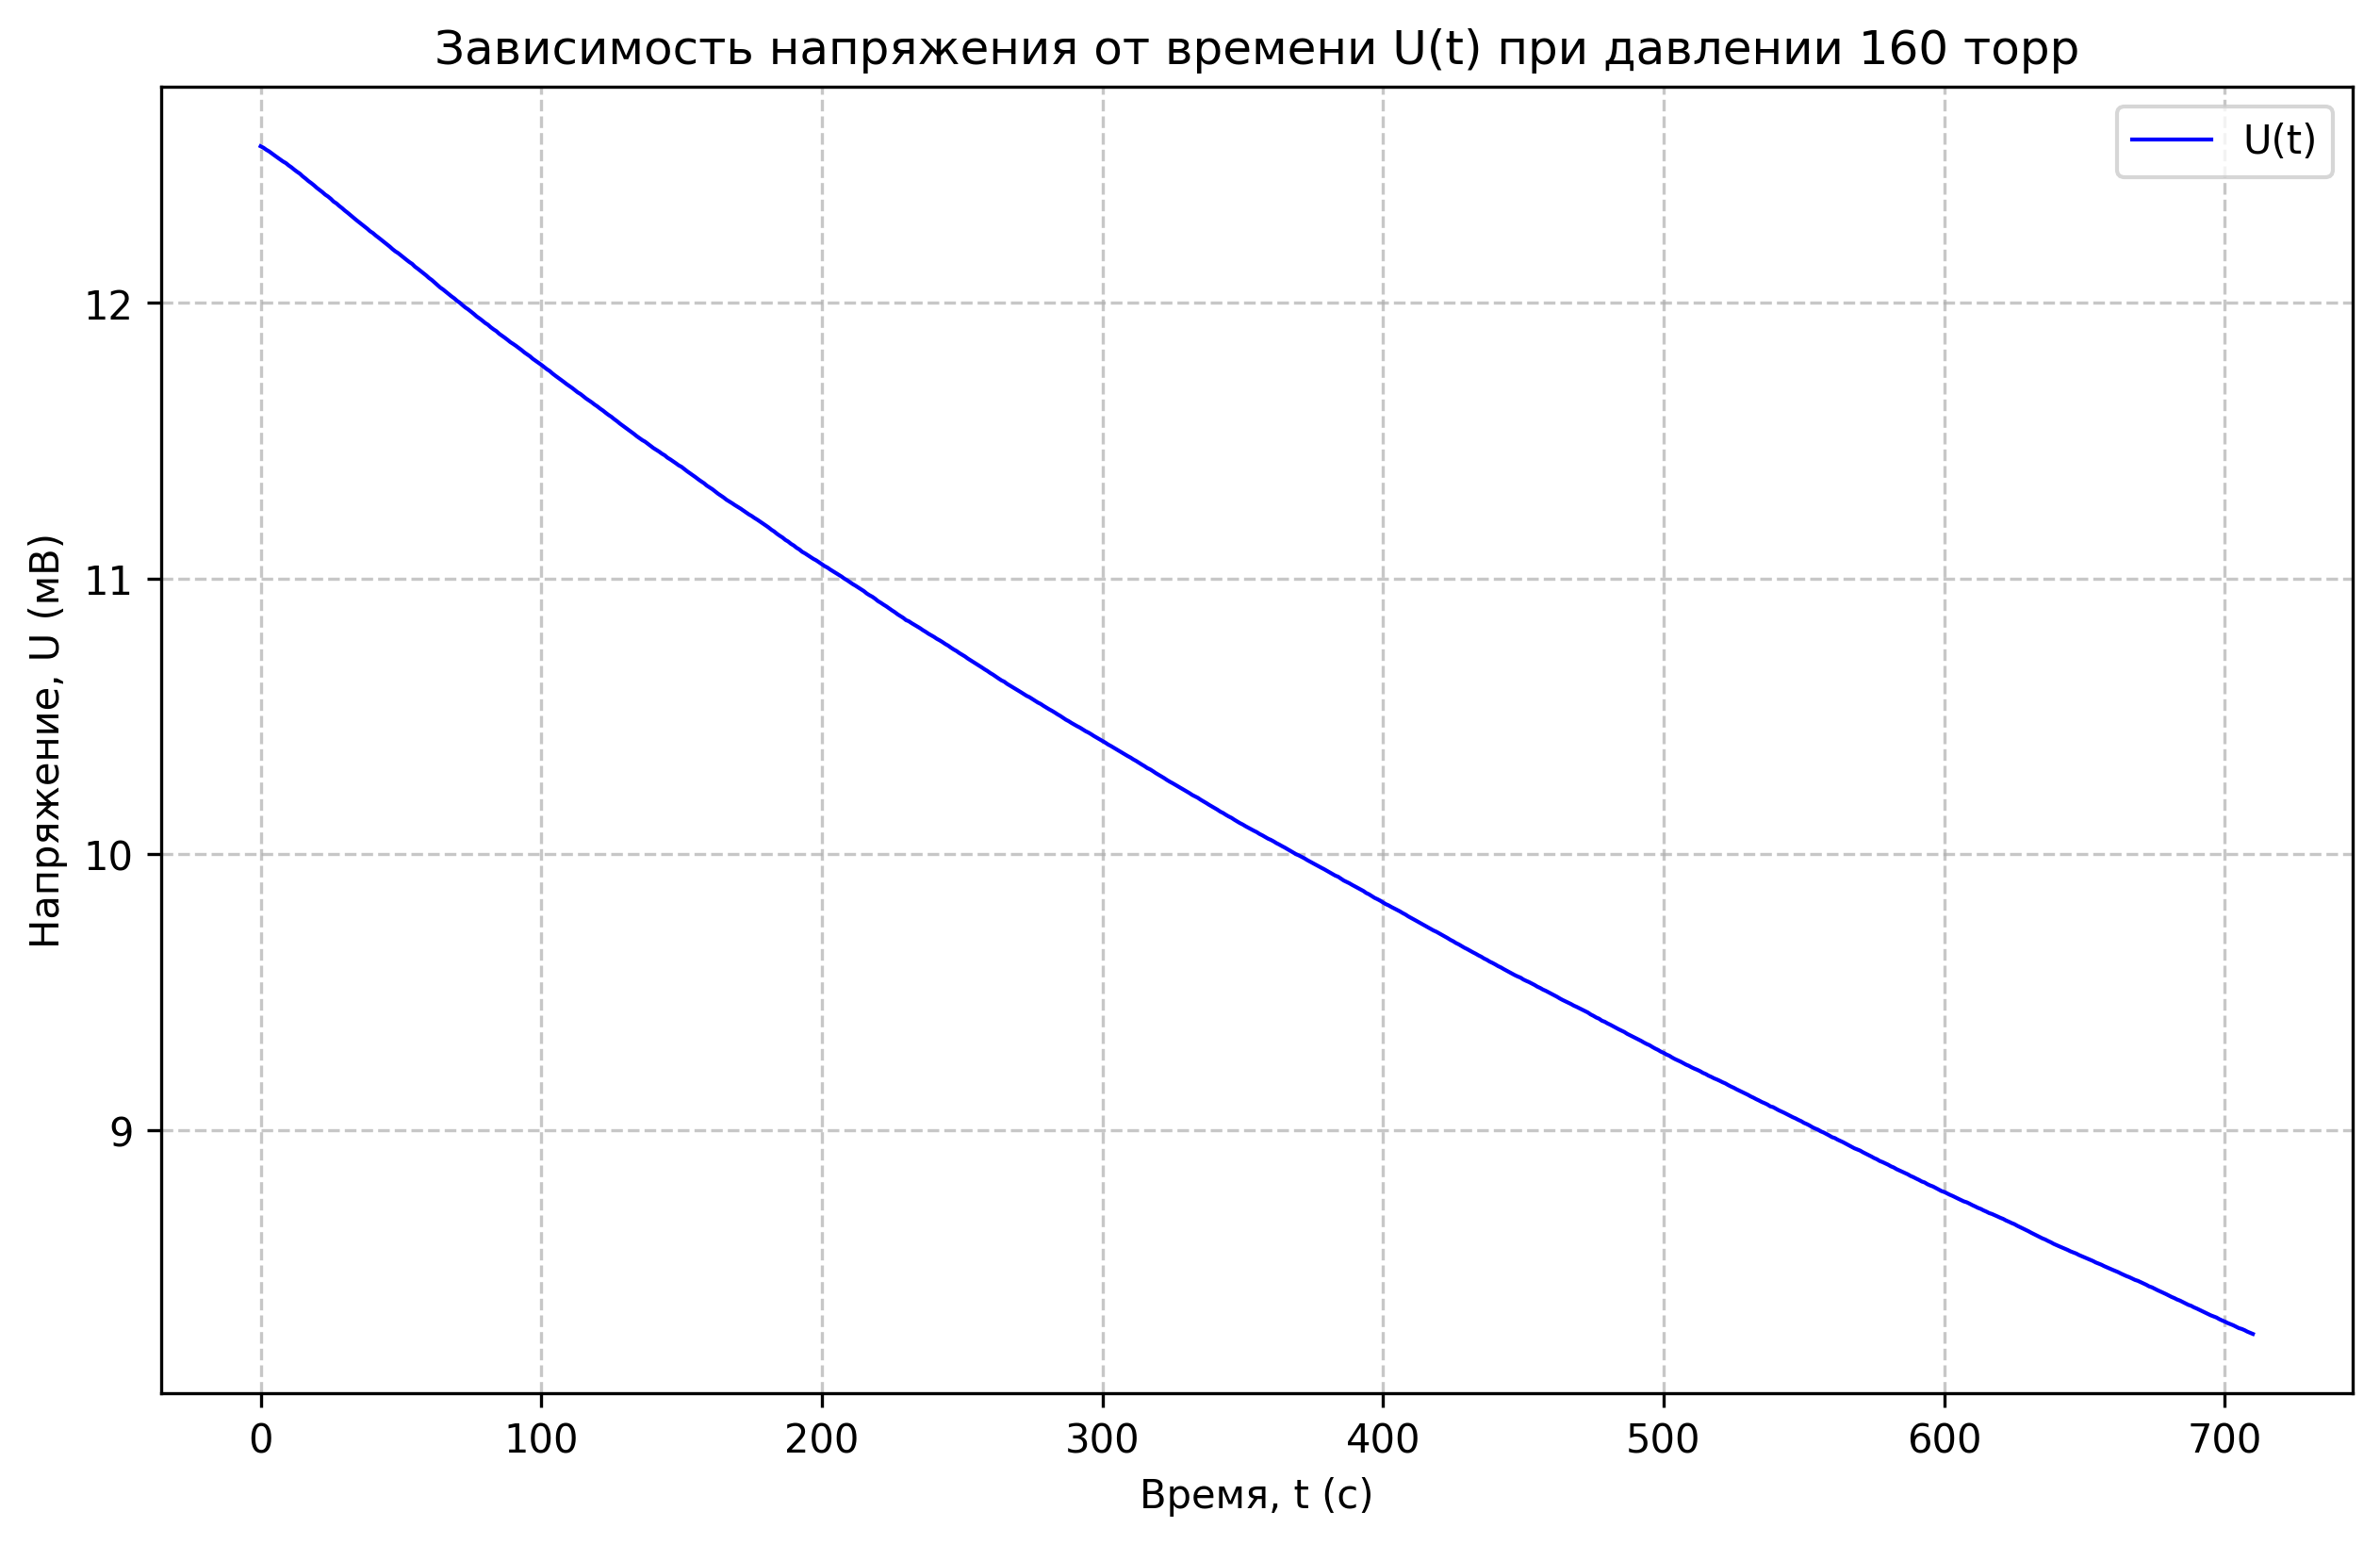
\includegraphics[width = \textwidth]{img/160.png}
Рис. 9. Зависимость напряжения от времени при давлении 160 торр.  
\end{figure}

